\begin{figure}[ht]
 \centering
 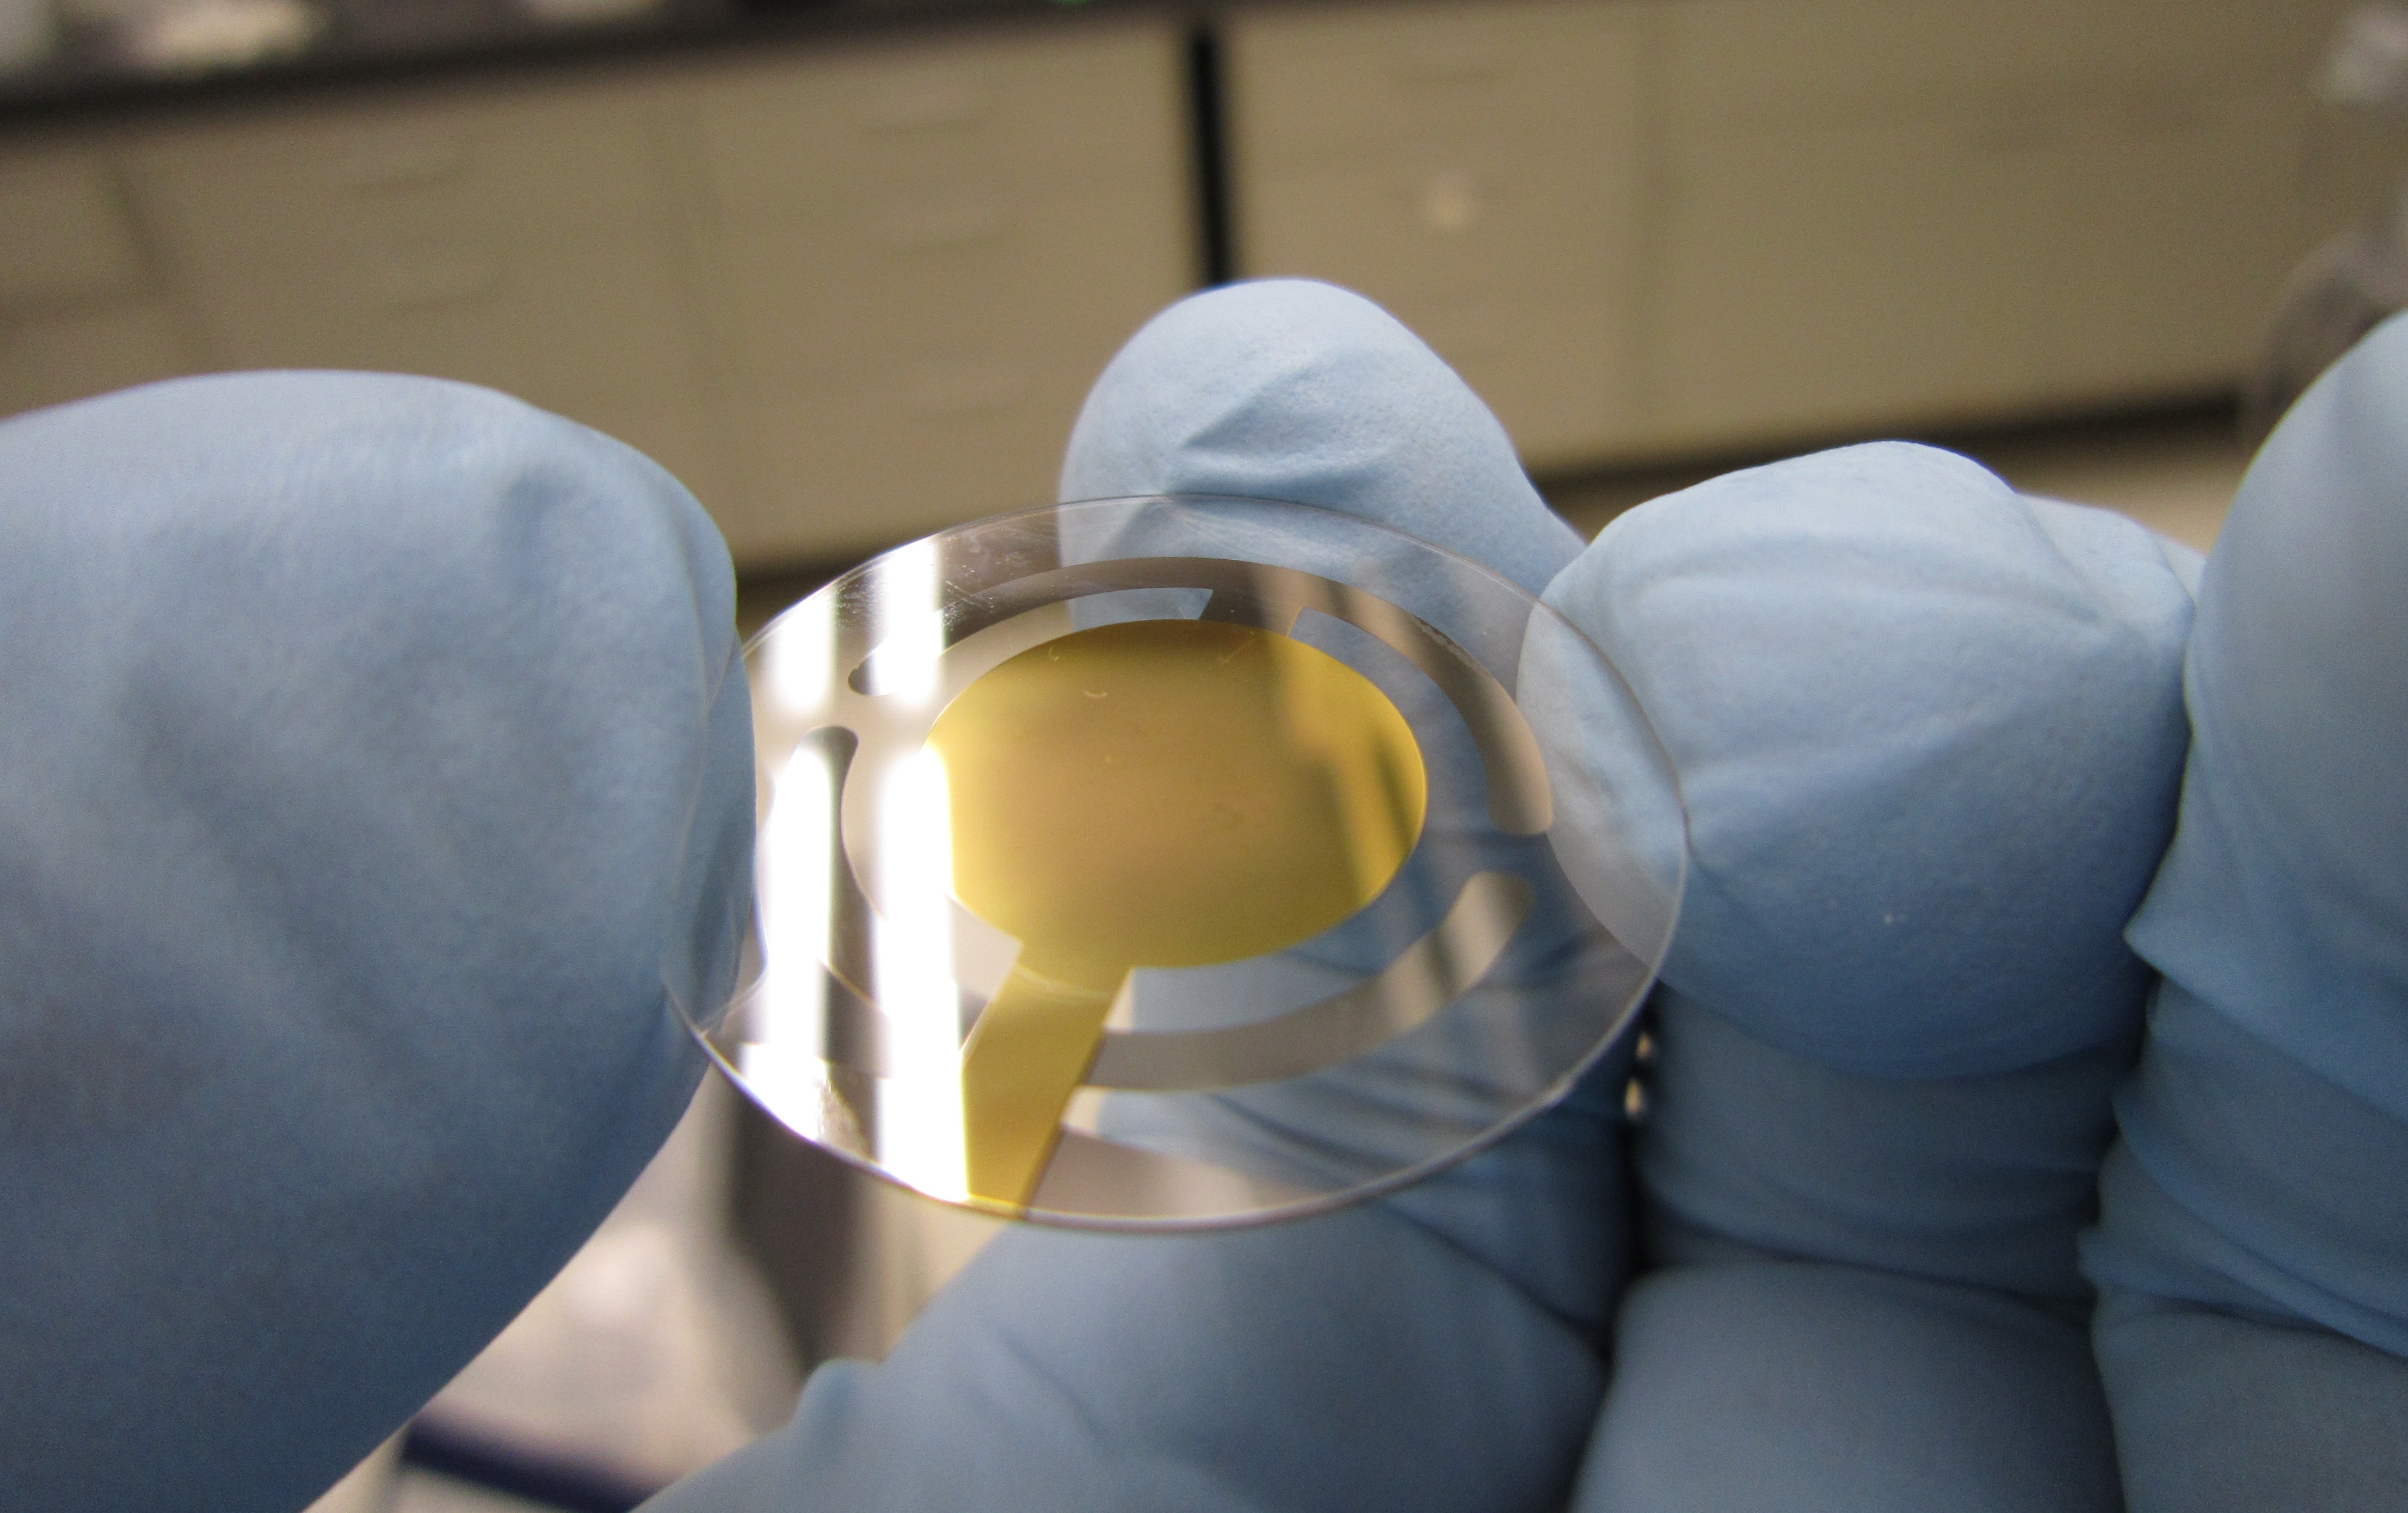
\includegraphics[keepaspectratio,width=12cm]{qcm/figures/qcm_holding.jpg}
 \caption{A \SI{25}{\milli\meter} \SI{5}{\mega\hertz} quartz crystal microbalance.}
\label{fig:qcmholding}
\end{figure}
There are few experimental techniques allowing application of force
on biological molecules. Among them, optical or magnetic tweezers and
atomic force microscopes (AFMs) have provided much insight into the
mechanics of molecules such as
DNA~\cite{cui2000pulling}~\cite{marko1995stretching}, improved
understanding of friction and wear in
proteins~\cite{suda2001origin}~\cite{bormuth2009protein}, and have even
been able to observe stepwise motion of motor
proteins~\cite{asbury2003kinesin}.

However powerful, these methods are not able to be deployed as integrated
devices to probe the mechanical properties of heterogeneous samples in a
wide range of applications; tweezer and AFM experiments rely on highly
trained experimentalists, are not widely applicable as analytical tools,
and are often constrained to the analysis of well prepared homogeneous
samples not amenable to multiplexing.

Among tools suitable for direct mechanical transduction, the quartz crystal
microbalance (QCM) has seen increasing real-world utility as a simple, cost
effective, and highly versatile mechanical biosensing platform. A QCM is
typically a thin disk-shaped piece of strategically cut piezoelectric
quartz with electrodes on either side. When part of an electronic
oscillator circuit, the quartz can form a mechanical resonator which
vibrates at certain fundamental frequencies. Changes in the fundamental
frequencies and their associated bandwidths upon sample adsorption or
desorption are related to the properties of the sample and the strength of
its coupling to the QCM. Since its introduction by
Sauerbrey~\cite{sauerbrey1959verwendung} in 1959 as sub-monolayer thin-film
mass sensors in the gas phase, the understanding of QCM sensors has been
repeatedly enhanced to study phenomena such as viscoelastic films in the
liquid phase~\cite{kanazawa1985frequency}, non-destructive contact
mechanics~\cite{johannsman2007contacts}, and complex topologies of
biopolymers and biomacromolecules~\cite{marx2003quartz}. 

Naturally, QCMs do not come without their own disadvantages. The underlying
mechanical properties of the sample are often not revealed by the stepwise
changes in the QCM sensorgram, an issue complicated by the choice of
theoretical model.  Operation of QCMs in the liquid phase is also
associated with a rather low-Q resonance, limiting their sensitivity and
precluding their use for single molecule detection.  Furthermore, up to now
it has not been possible to integrate the application of force on
biomolecules in QCM measurements.

In light of these issues and the analytical power of force based
techniques, herein is described a novel type of instrument using a QCM as a
direct mechanical transducer for the response of discrete samples
(molecules, particles) placed in a variable force field provided by a
standard commercial centrifuge.  This \textit{centrifugal force quartz
crystal microbalance} (CF-QCM) concept is concerned with direct
introduction of pico to nanoscale forces in the liquid phase for analyzing
the mechanical properties of biomaterials.

%\subsection{Organization}
%This chapter begins with a small historical perspective and proceeds
%with a derivation of the relevant mathematics which will allow the
%prediction of the response of a QCM for samples under centrifugal force.
%Subsequently, \Chapter{ch:qcmexperimental} outlines the technical details of the
%CF-QCM; hardware, electronics, and data acquisition.  Drawing on the theory
%presented, the main results of this work are presented in
%\Chapter{ch:qcmloadsituations} for different types of samples.  A
%finite element simulation was also employed to compliment the
%theoretical model.  The simulation is presented in
%\Chapter{ch:qcmsimulation} along with predictions of CF-QCM behavior for
%samples which have not yet been subjected to experiment.
